\chapter{Parametric Exploration of the \emph{EvoTSC} Model}
\label{chap:param}

In this chapter, I present several sets of additional evolutionary simulations.
In these simulations, I explore the robustness of the characteristics of evolved populations to variations in the model, measuring whether they are able to evolve differentiated gene expression patterns as a response to different environments, and comparing their speed of evolution with that of the main runs presented in Chapter~\ref{chap:ploscb}.
Rather than change parameters directly related to the effect of supercoiling on transcription as in Section\ref{sec:alife:param_explor} (which uses the simple model), I changed parameters related to the structure of the genomes: the maximum interaction distance between genes, and the mean intergenic distance.
I also tested the sensitivity of the model to smaller changes in the environment, by changing $\sigma_A$ and $\sigma_B$.
These additional simulations were run for 250,000 generations, as the trends that we are interested in are already clearly visible by that stage, and were replicated 15 (instead of 30) times each.
The characteristics of these runs are summarized in Table~\ref{tab:param:params}.


\begin{table}[H]
\begin{center}
\begin{tabular}{l c r r}
\toprule
\textbf{Parameter} & \textbf{Symbol} & \textbf{Value} & \textbf{Replicates} \\
\midrule
Interaction distance & $d_{max}$ & \textbf{5 kb} & \textbf{30}\\
& & 25 kb & 15\\
\midrule
& & 10 & 15\\
Mean intergenic distance & $d_0$ & \textbf{125} & \textbf{30} \\
& & 1,000 & 15\\
& & 10,000 & 5 \\
\midrule
& & 0.0001 & 5\\
Environment supercoiling & $\delta\sigma_{A/B}$ & 0.001 & 5\\
& & \textbf{0.01} & \textbf{30}\\
\bottomrule
\end{tabular}
\end{center}
\caption[Table of parameter values explored in additional \emph{EvoTSC} simulations]{Table of the parameters and associated values explored in additional experiments (separated by horizontal lines).
For each experiment, the row in bold font corresponds to the parameter values used in the main run described in Chapter~\ref{chap:ploscb}, and is shown for reference.}
\label{tab:param:params}
\end{table}

In order to see the result of slightly more realistic simulations, I also ran a set of simulations with a higher number of genes (300 instead of 60).
Finally, I also ran simulations with an additional mutational operator: mutations in the intergenic distances, corresponding to indels in the non-coding regions of the genome.

\section{Interaction Distance}

The size of the topological domains of bacterial DNA, inside which supercoiling can freely propagate, has historically been estimated to be on the order of a few thousand base pairs~\citep{elhanafi2000,kouzine2013}, but recent work has suggested that the could be up to ten times higher~\citep{visser2022}.
As this distance sets a limit to the number of genes that can interact through the transcription-supercoiling coupling, it plays an important role in the structure of the gene regulatory network that emerges from the coupling.

A higher interaction distance increases the number of interacting genes, and could therefore make genomic inversions more deleterious by making them disrupt a larger part of the regulatory network.
In order to test this hypothesis, I ran a set of 15 simulations in which the interaction distance $d_{max}$ was set to 25kb, as measured in~\citep{visser2022}, for 1,000,000 generations.

As Figure~\ref{fig:param:inter25k-finess} shows, populations in these runs reach an average fitness of around $10^{-3}$ by the end of the simulations, as in the default evolutionary run (see Figure~\ref{fig:ploscb:main_fitness}).
In this case, the larger interaction distance do

\begin{figure}[H]
\centering
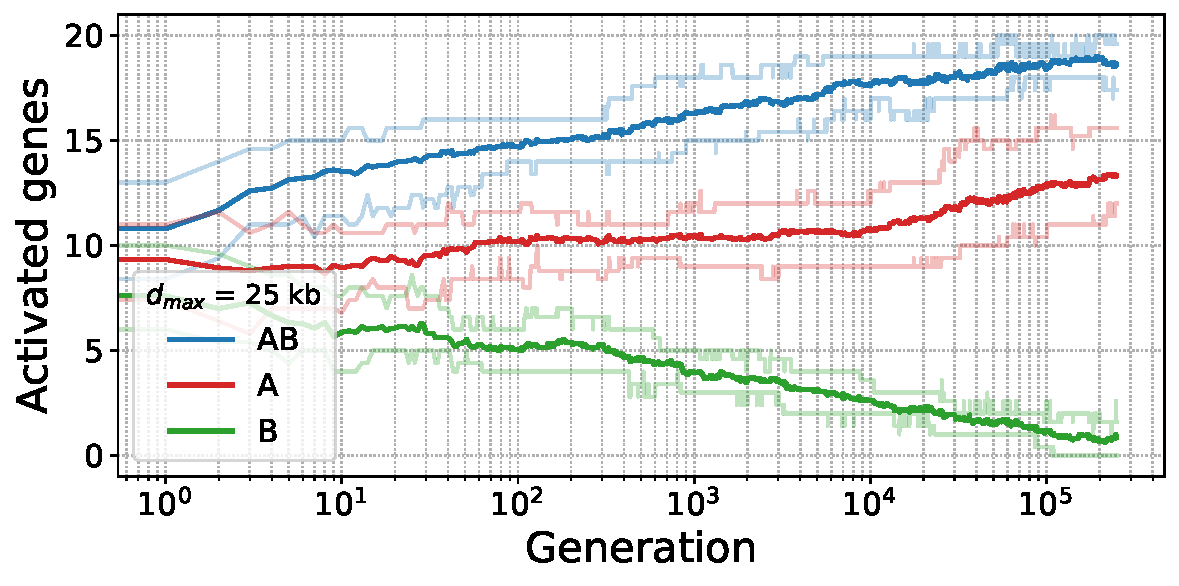
\includegraphics[width=0.49\textwidth]{param/interaction-25k/gene_activity_env_A.pdf}
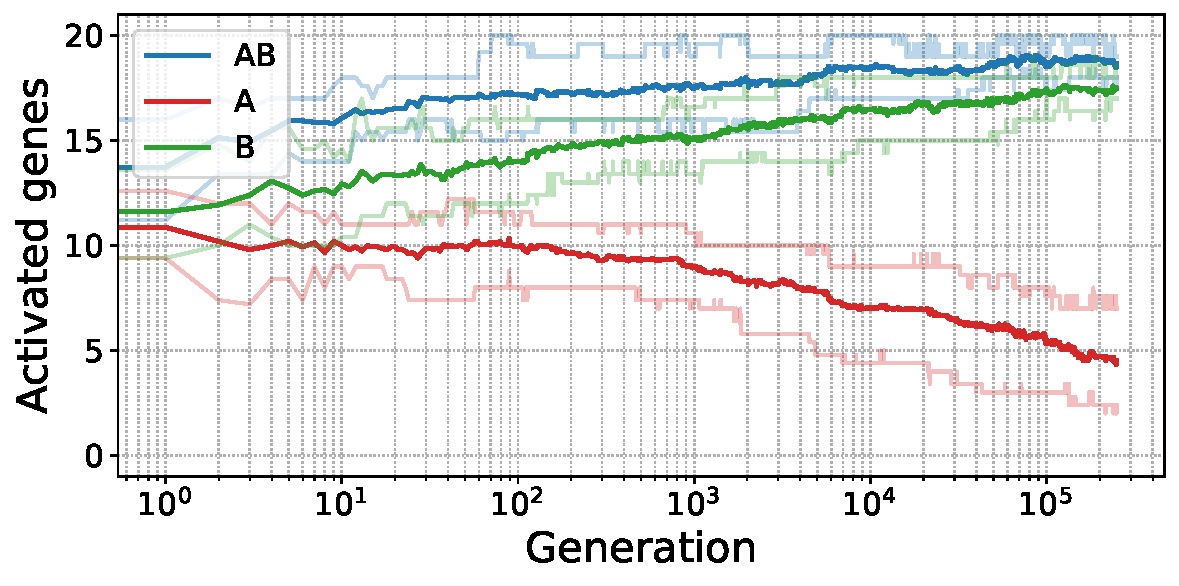
\includegraphics[width=0.49\textwidth]{param/interaction-25k/gene_activity_env_B.pdf}
\caption[Evolution of the number of active genes in each environment with an interaction distance of 25 kb]{Evolution of the number of active genes in environment A (left) and environment B (right), with an interaction distance of 25 kb.}
\label{fig:param:inter25k-active}
\end{figure}


\begin{figure}[H]
\centering
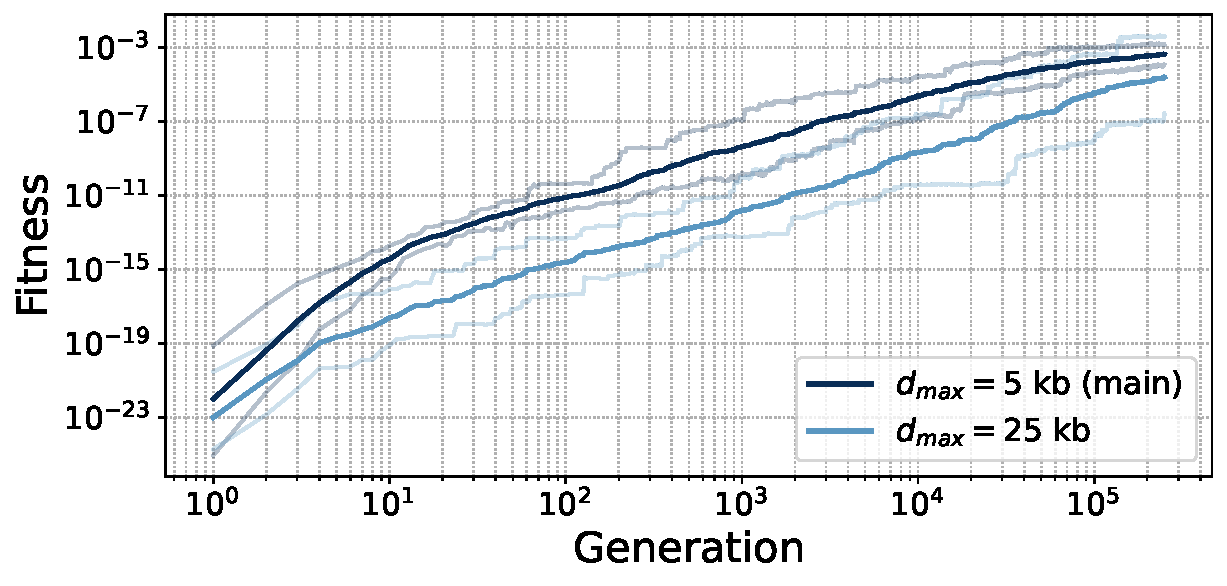
\includegraphics[width=0.75\textwidth]{param/interaction-25k/fitness_all_with_main.pdf}
\caption[Average fitness during evolution, with an interaction distance of 25 kb]{Average fitness during evolution with an interaction distance of 25 kb and 5 kb for comparison.}
\label{fig:param:inter25k-finess}
\end{figure}

\begin{figure}[H]
\centering
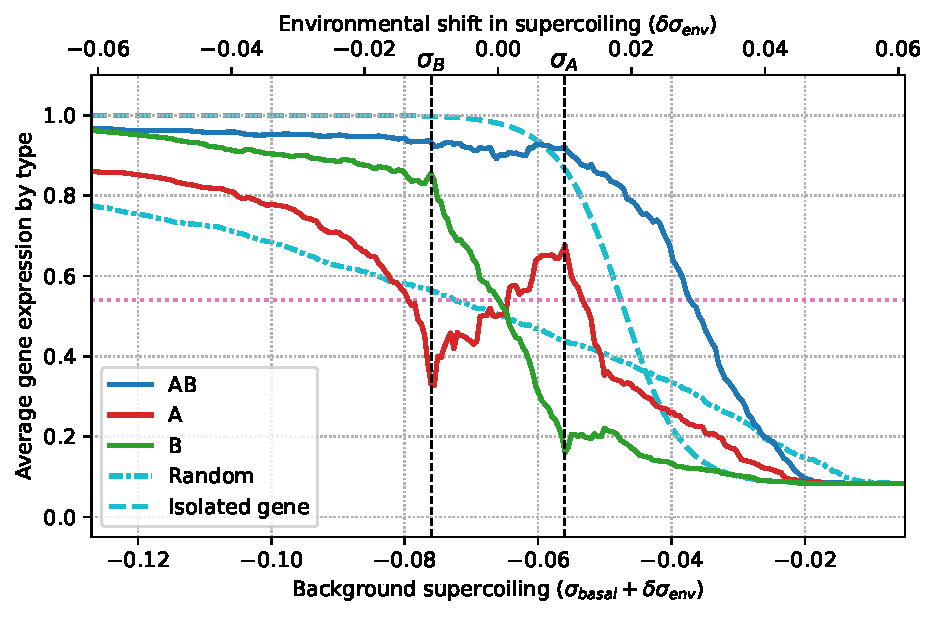
\includegraphics[width=\textwidth]{param/interaction-25k/activity_sigmas_avg.pdf}
\caption[Average gene expression as a function of background supercoiling, with an interaction distance of 25 kb]{Average gene expression as a function of background supercoiling, with an interaction distance of 25 kb.}
\label{fig:param:inter25k-activ-by-sigma}
\end{figure}

\FloatBlock






\section{Mean Intergenic Size}

\begin{figure}
\centering
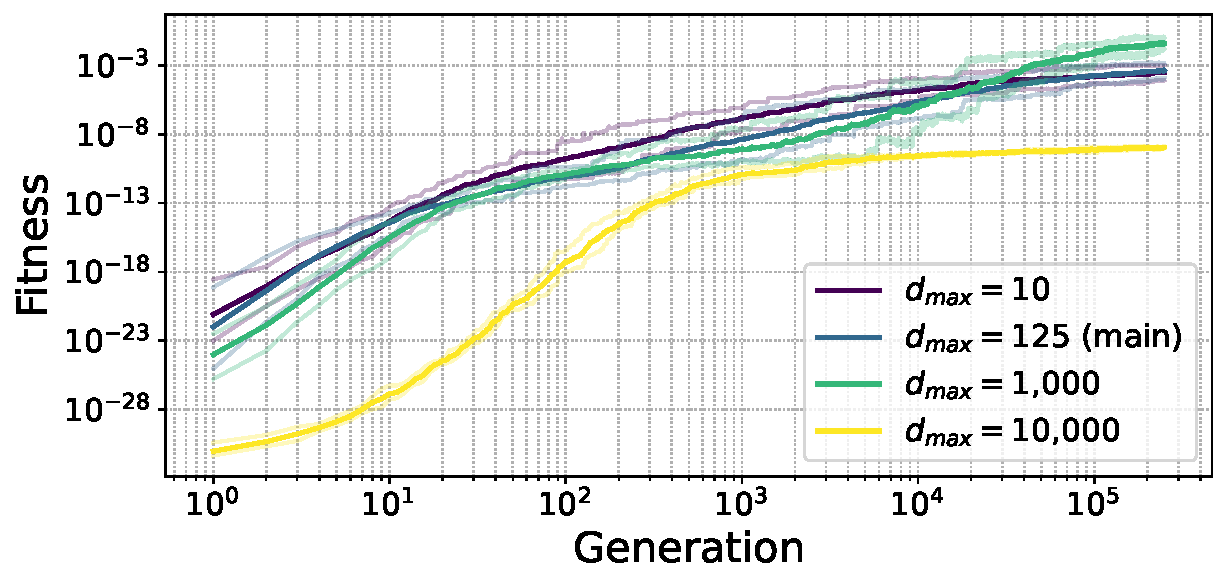
\includegraphics[width=0.75\textwidth]{param/mean-intergene/fitness_all_with_main.pdf}
\caption{Evolution of the fitness during evolution for average intergenic sizes of 10 bp \textbf{REFAIRE AVEC 15 REP}, 125 bp (main run), 1,000 bp, and 10,000 bp.}
%\label{}
\end{figure}

\begin{figure}
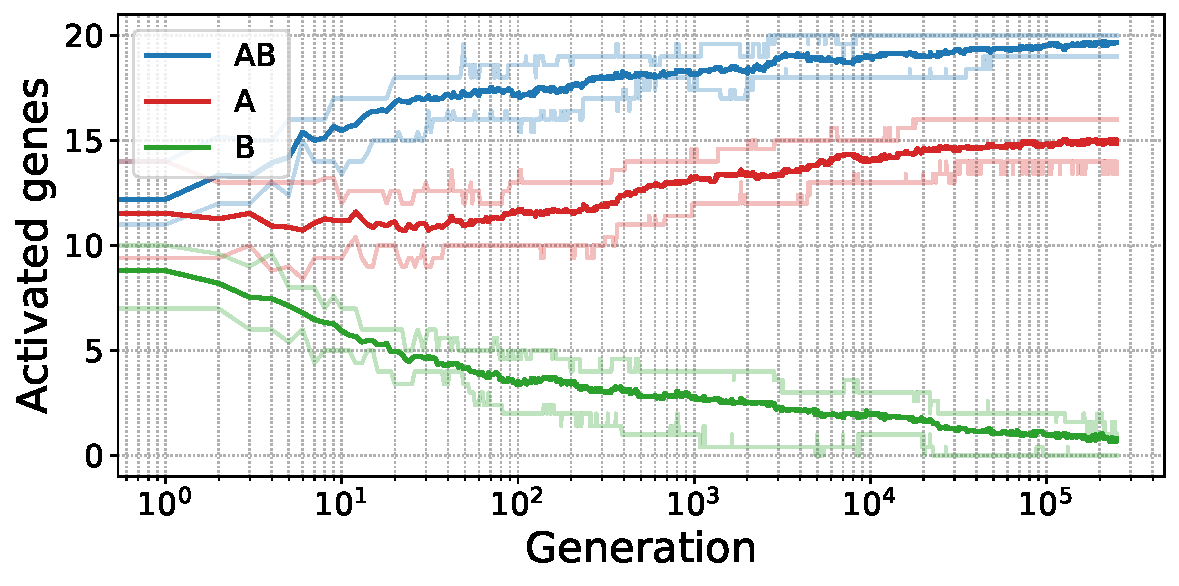
\includegraphics[width=0.49\textwidth]{param/mean-intergene/inter-0.01k/gene_activity_env_A.pdf}
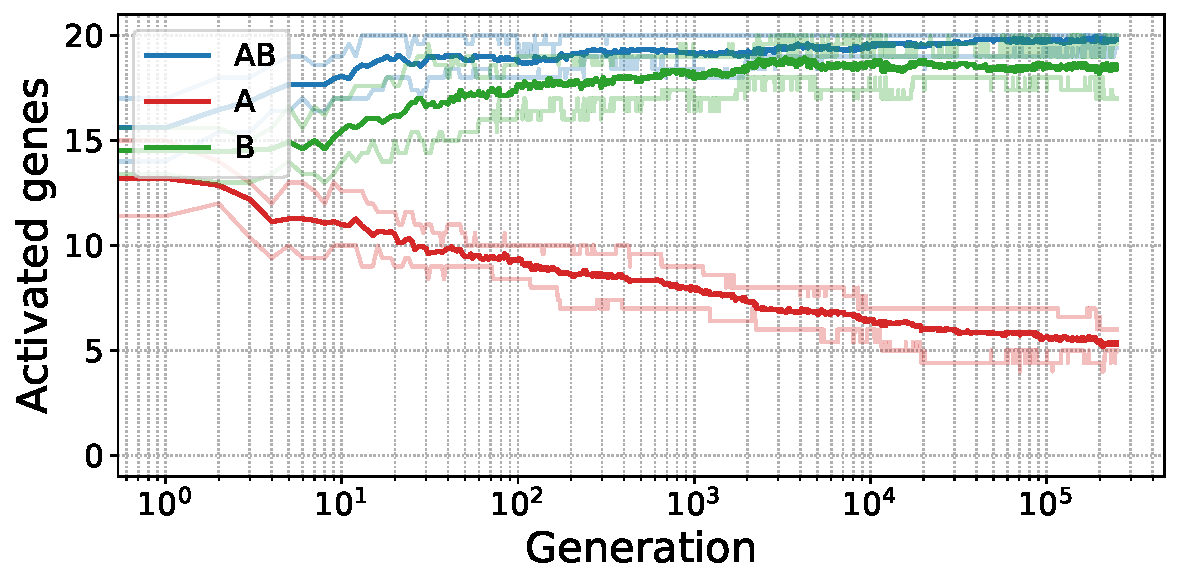
\includegraphics[width=0.49\textwidth]{param/mean-intergene/inter-0.01k/gene_activity_env_B.pdf}

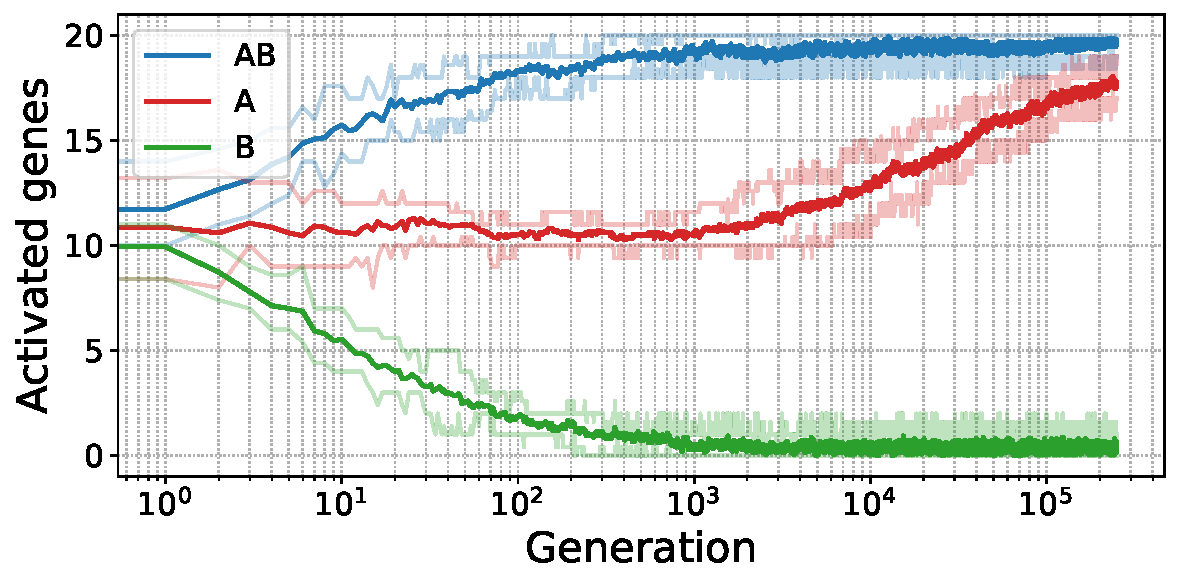
\includegraphics[width=0.49\textwidth]{param/mean-intergene/inter-1k/gene_activity_env_A.pdf}
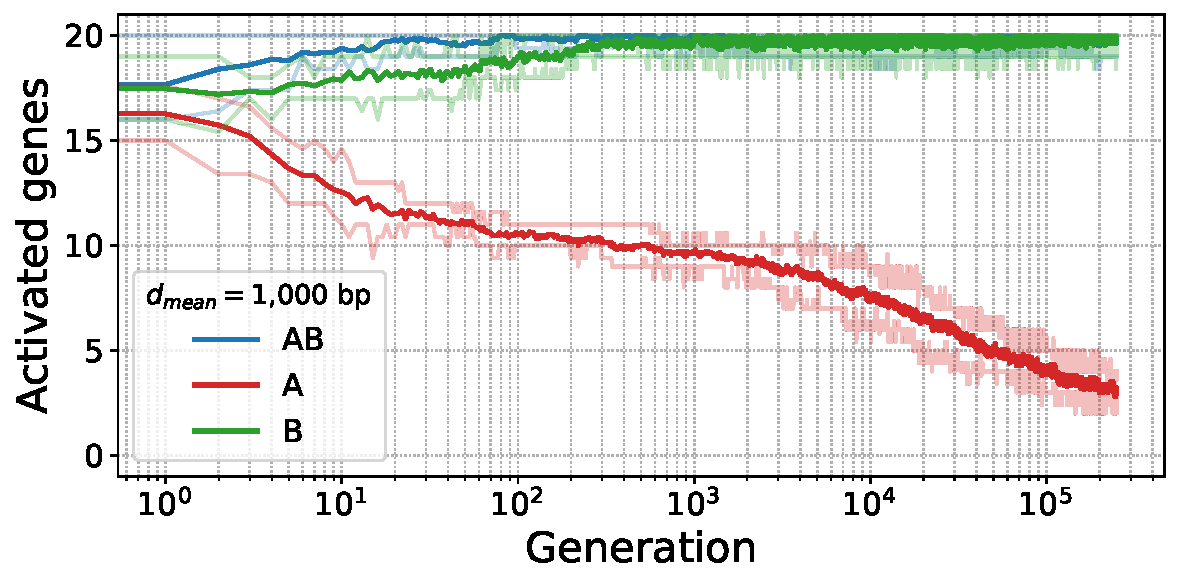
\includegraphics[width=0.49\textwidth]{param/mean-intergene/inter-1k/gene_activity_env_B.pdf}

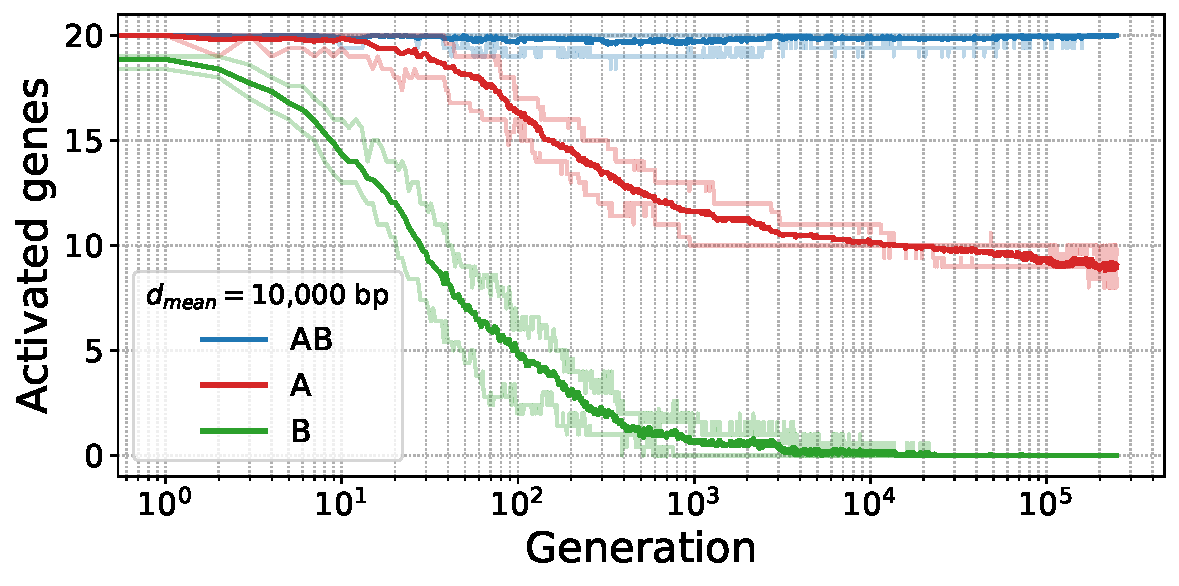
\includegraphics[width=0.49\textwidth]{param/mean-intergene/inter-10k/gene_activity_env_A.pdf}
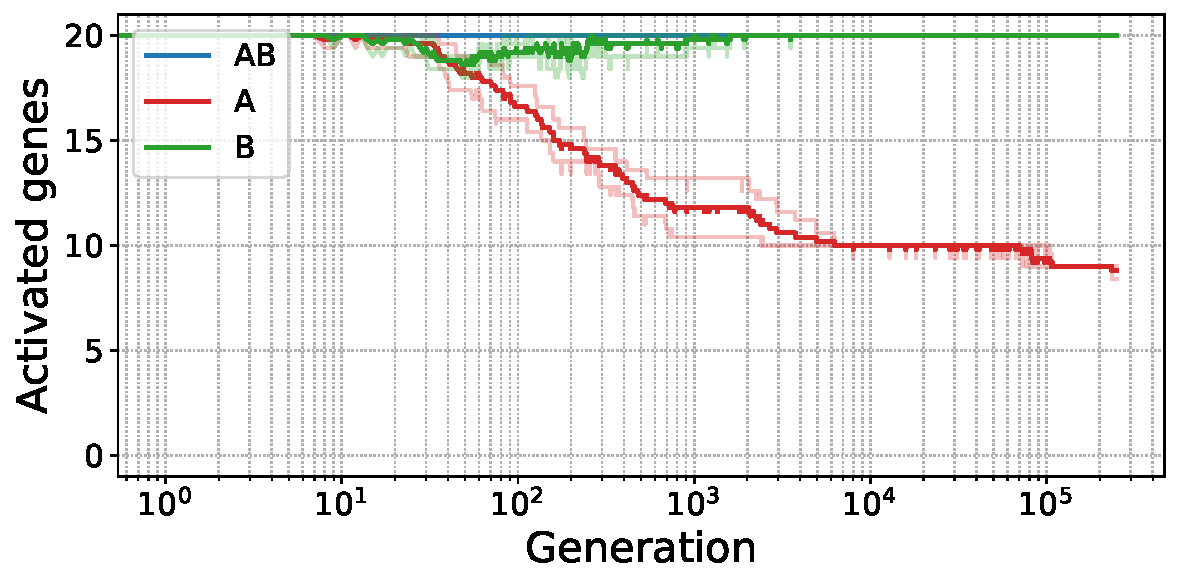
\includegraphics[width=0.49\textwidth]{param/mean-intergene/inter-10k/gene_activity_env_B.pdf}
\caption{Evolution of the number of activated genes in environment A (left) and B (right) during evolution, for average intergenic sizes of 10 bp (top) \textbf{REFAIRE AVEC 15 REP}, 1,000 bp (middle), and 10,000 bp (bottom) base pairs.}
%\label{}
\end{figure}

\begin{figure}

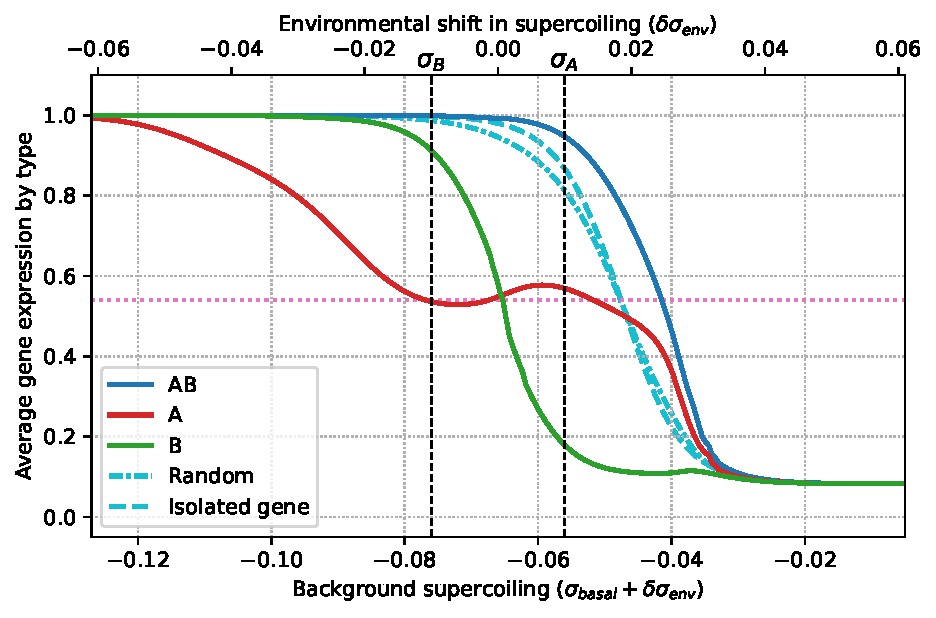
\includegraphics[width=\textwidth]{param/mean-intergene/inter-10k/activity_sigmas_avg.pdf}
\caption{Average gene expression as a function of background supercoiling, with an intergenic distance of 10 kb.}
\end{figure}


\begin{figure}

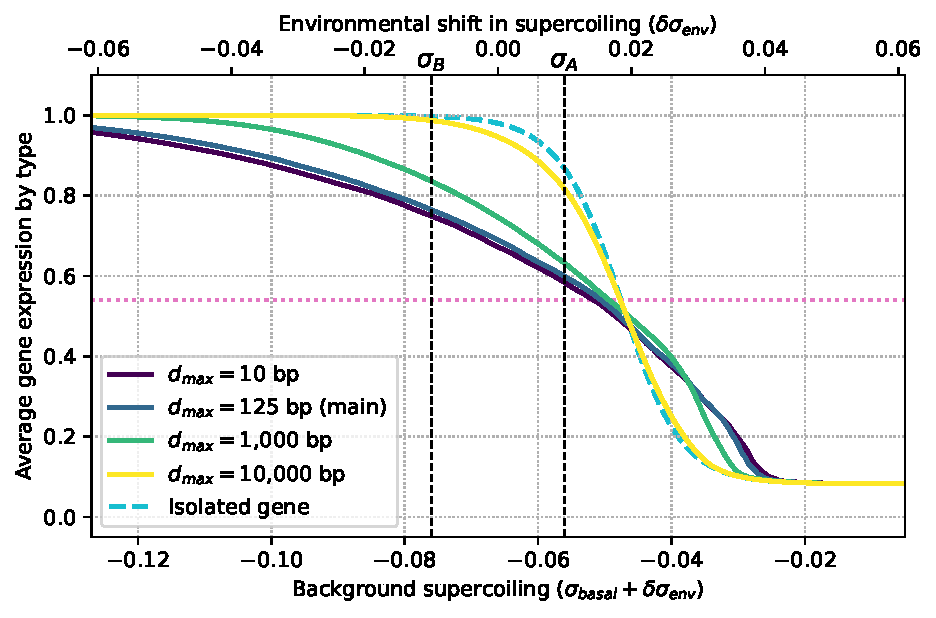
\includegraphics[width=\textwidth]{param/mean-intergene/random_activ_per_sigma.pdf}
\caption{expression level of random genes.}
\end{figure}








\FloatBlock

\section{Environmental Shift in Supercoiling}

\begin{figure}
\centering
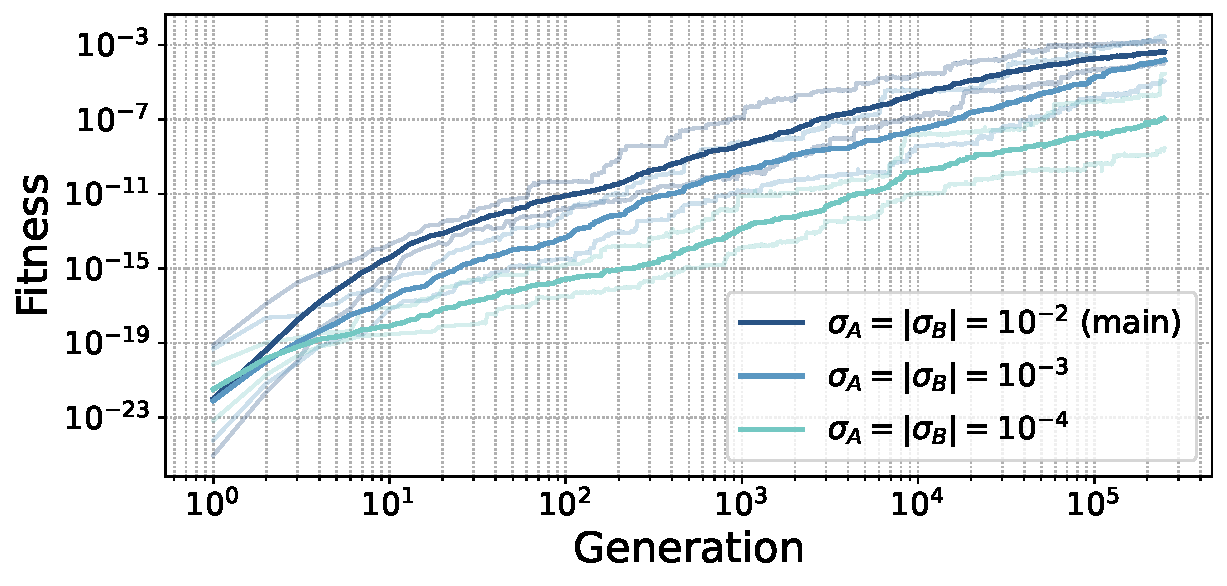
\includegraphics[width=0.75\textwidth]{param/sigma/fitness_all_with_main.pdf}
\caption{Evolution of the fitness during evolution for with environmental supercoiling shifts $\sigma_A = 0.001$ and $\sigma_B = -0.001$ (top) and $\sigma_A = 0.001$ and $\sigma_B = -0.001$ (bottom) \textbf{REFAIRE AVEC 15 REP}.}
%\label{}
\end{figure}


\begin{figure}
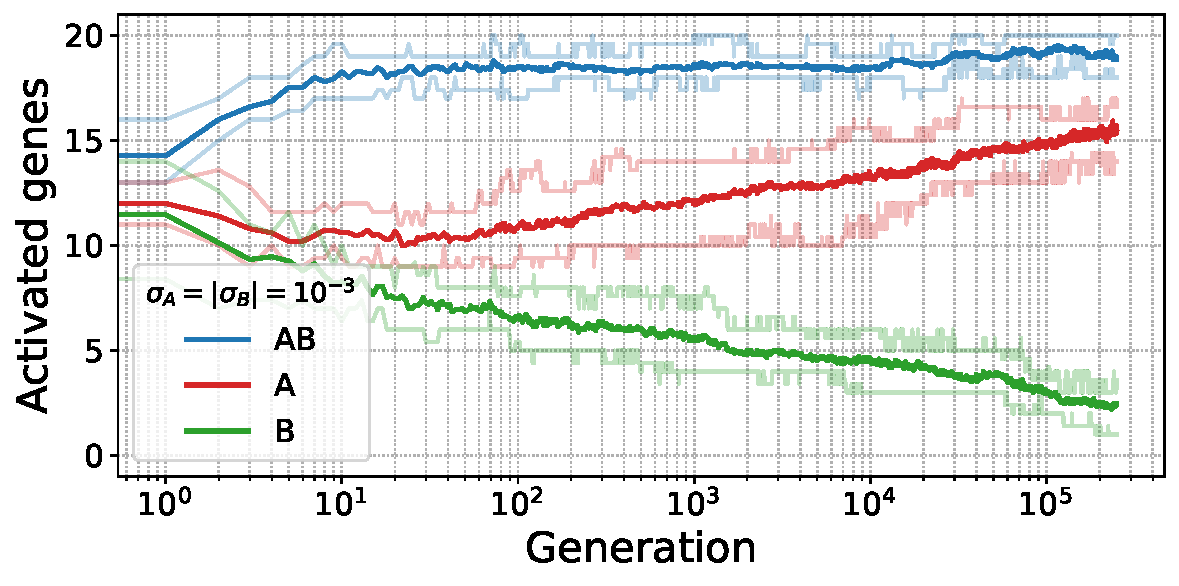
\includegraphics[width=0.49\textwidth]{param/sigma/sigma-1e-3/gene_activity_env_A.pdf}
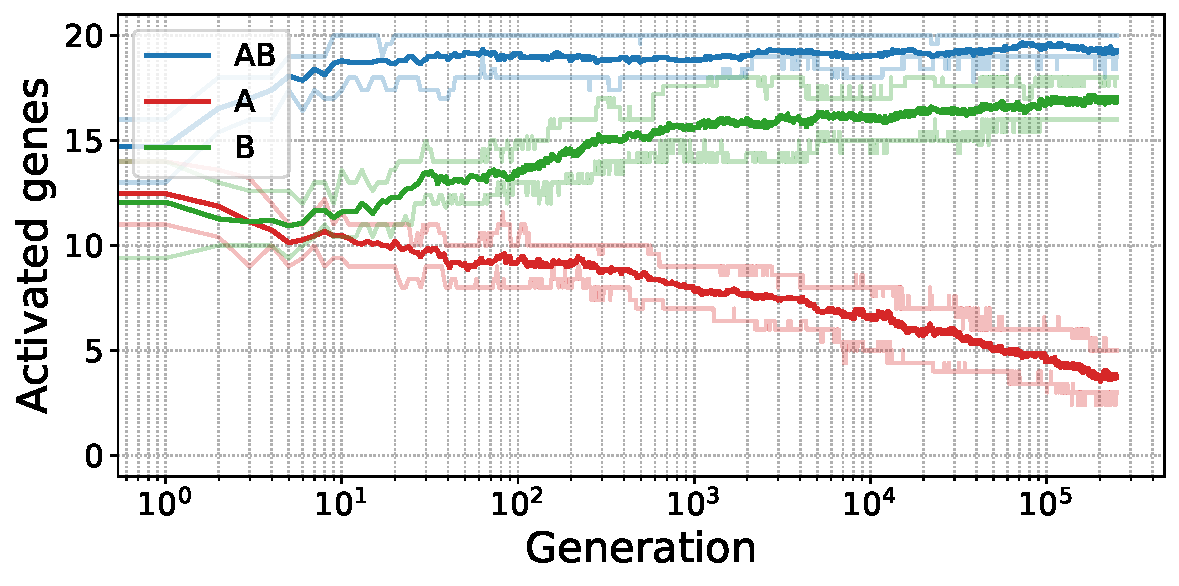
\includegraphics[width=0.49\textwidth]{param/sigma/sigma-1e-3/gene_activity_env_B.pdf}

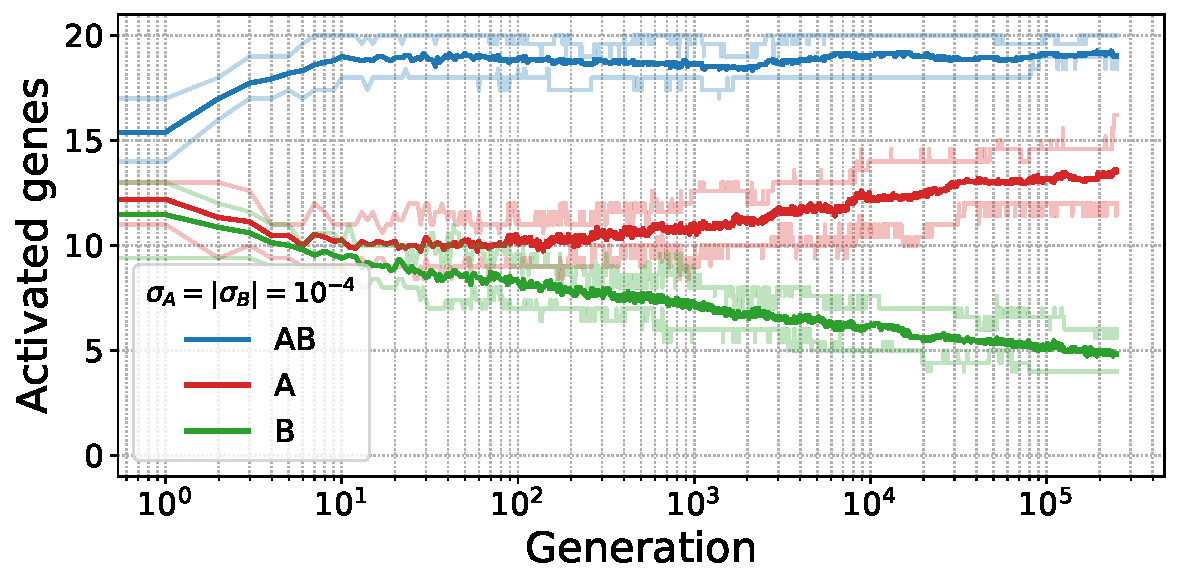
\includegraphics[width=0.49\textwidth]{param/sigma/sigma-1e-4/gene_activity_env_A.pdf}
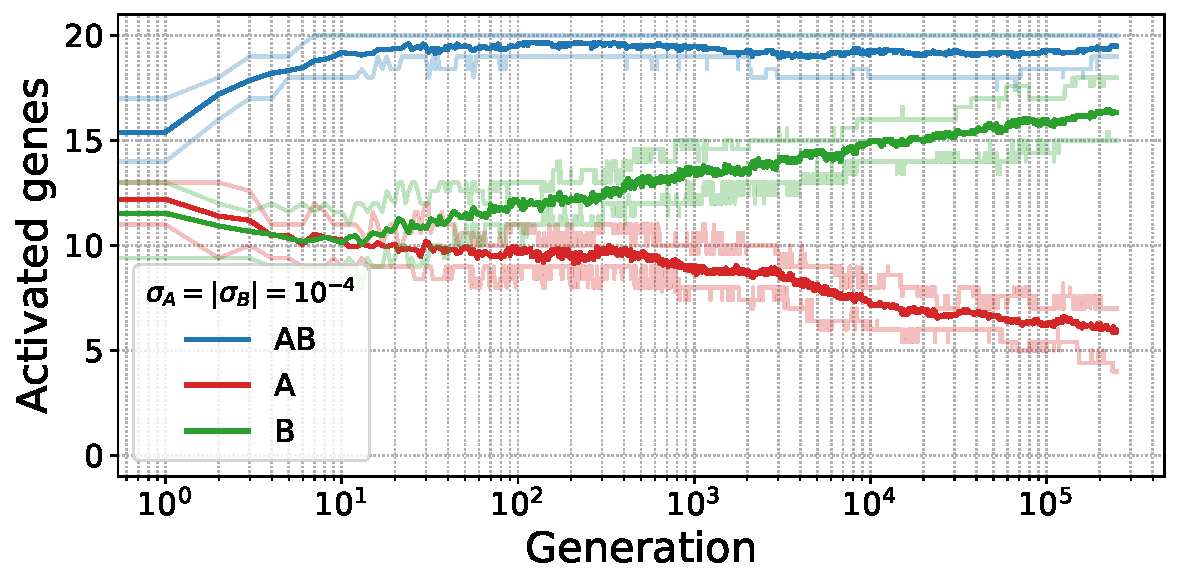
\includegraphics[width=0.49\textwidth]{param/sigma/sigma-1e-4/gene_activity_env_B.pdf}
\caption[Evolution of the number of active genes in each environment with an absolute environmental supercoiling shift of 0.001 or 0.0001]{Evolution of the number of active genes in environment A (left) and environment B (right), with environmental supercoiling shifts $\sigma_A = 0.001$ and $\sigma_B = -0.001$ (top) and $\sigma_A = 0.001$ and $\sigma_B = -0.001$ (bottom). \textbf{RELANCER AVEC 15 REP}}
\label{}
\end{figure}

Evolution still works with a 10 times or 100 times smaller shift in supercoiling caused by the environment.

\begin{figure}
\centering
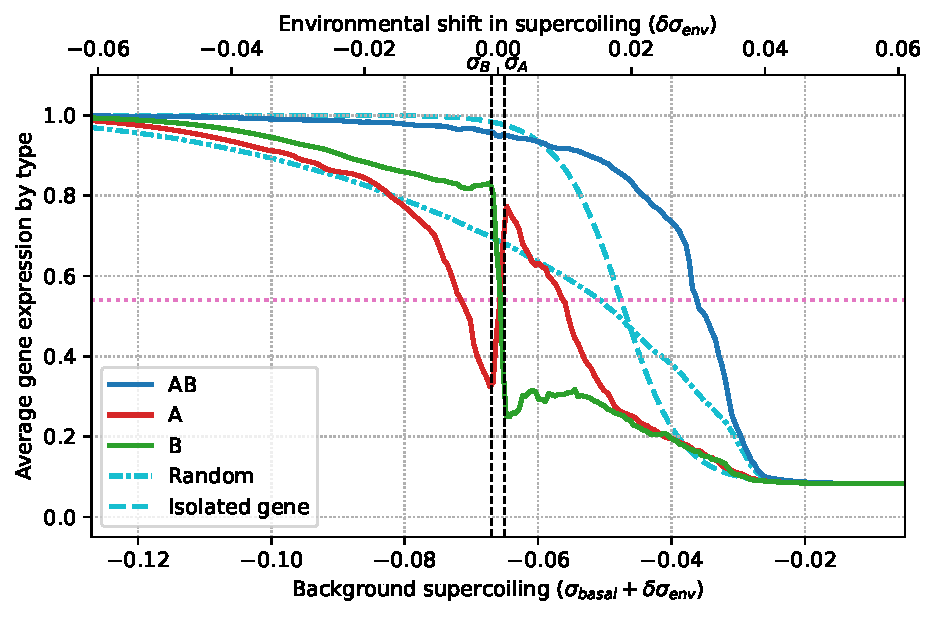
\includegraphics[width=\textwidth]{param/sigma/sigma-1e-3/activity_sigmas_avg.pdf}
\caption[Average gene expression as a function of background supercoiling, with an absolute environmental supercoiling shift of 0.001]{Average gene expression as a function of background supercoiling, with environmental supercoiling shifts $\sigma_A = 0.001$ and $\sigma_B = -0.001$.\textbf{RELANCER AVEC 15 REP}}
\end{figure}

\begin{figure}
\centering
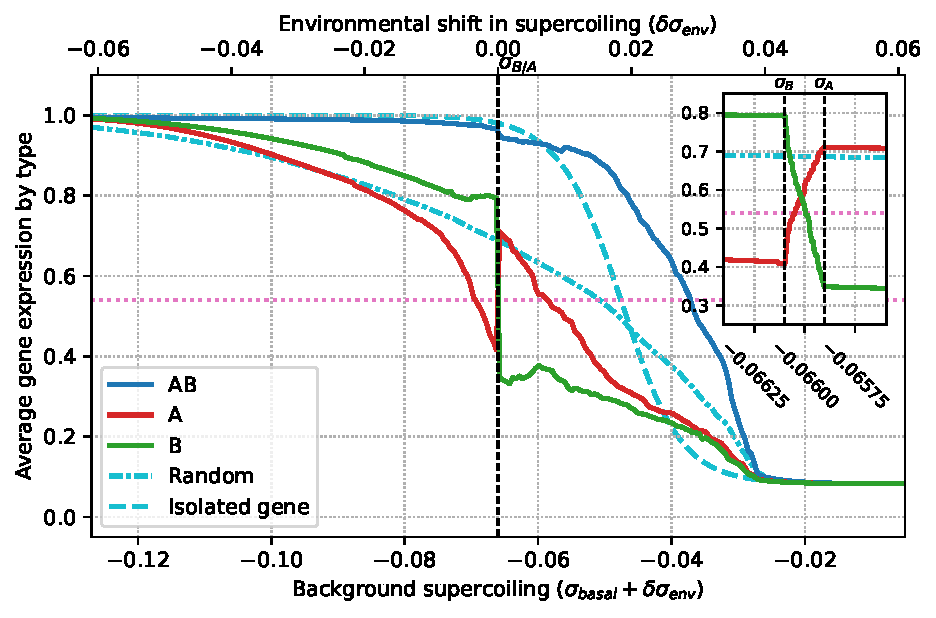
\includegraphics[width=\textwidth]{param/sigma/sigma-1e-4/activity_sigmas_avg.pdf}
\caption[Average gene expression as a function of background supercoiling, with an absolute environmental supercoiling shift of 0.0001]{Average gene expression as a function of background supercoiling, with environmental supercoiling shifts $\sigma_A = 0.0001$ and $\sigma_B = -0.0001$.\textbf{RELANCER AVEC 15 REP}}
\end{figure}

In all these cases, everything still works.






\FloatBlock

\section{Number of Genes}

\begin{figure}[H]
\centering
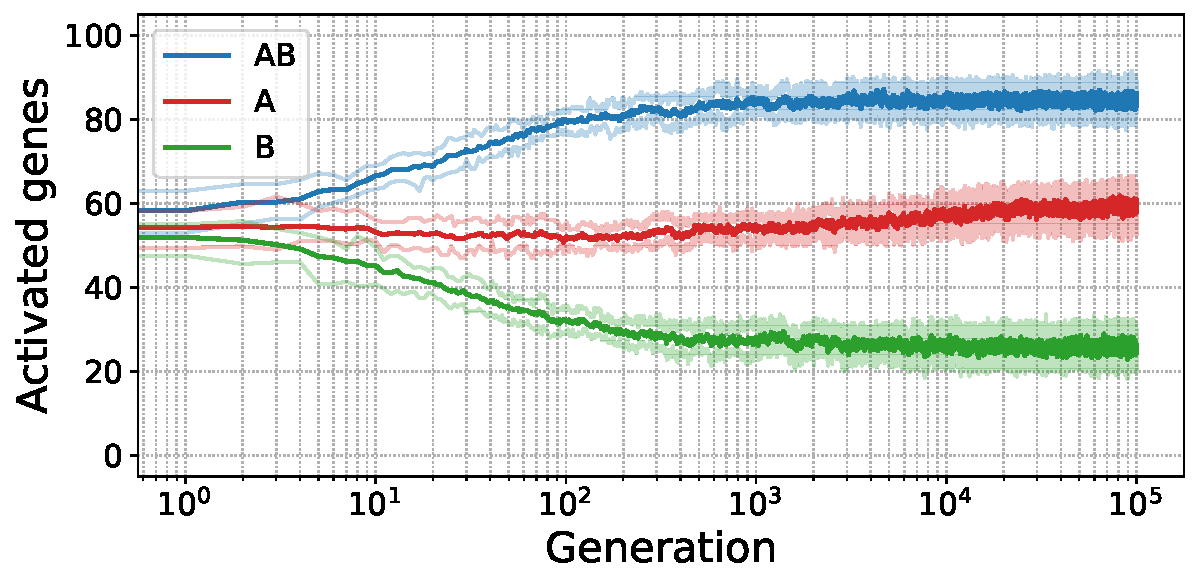
\includegraphics[width=0.49\textwidth]{param/300-genes/gene_activity_env_A.pdf}
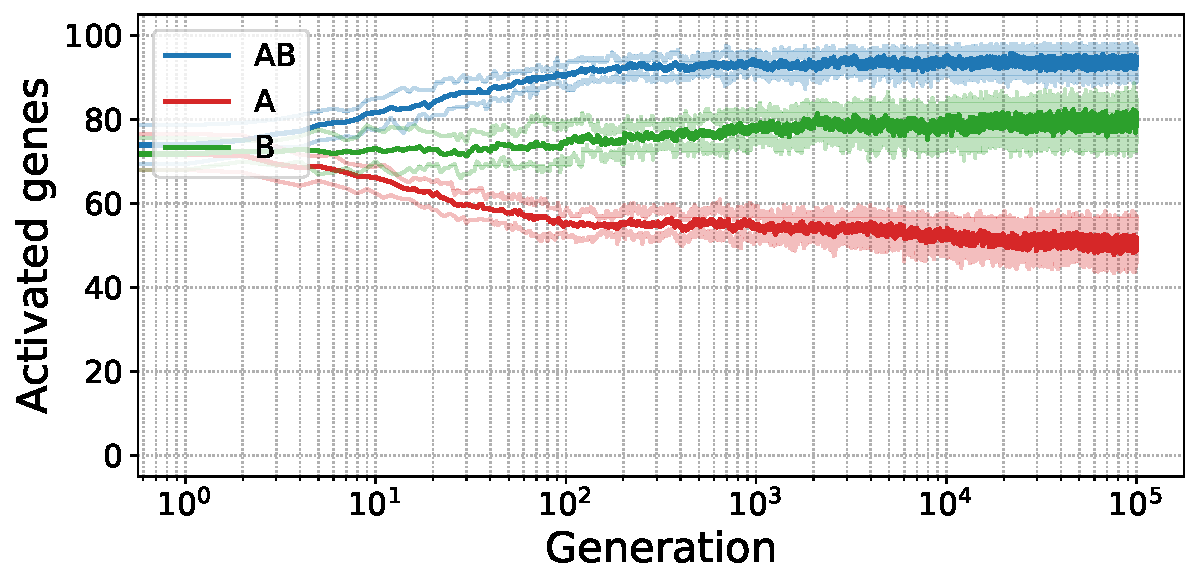
\includegraphics[width=0.49\textwidth]{param/300-genes/gene_activity_env_B.pdf}
\caption[Evolution of the number of active genes in each environment, with a 300-gene genome]{Evolution of the number of active genes in environment A (top) and environment B (bottom), with an interaction distance of 25 kb.}
%\label{fig:param:inter25k-active}
\end{figure}

\begin{figure}[H]
\centering
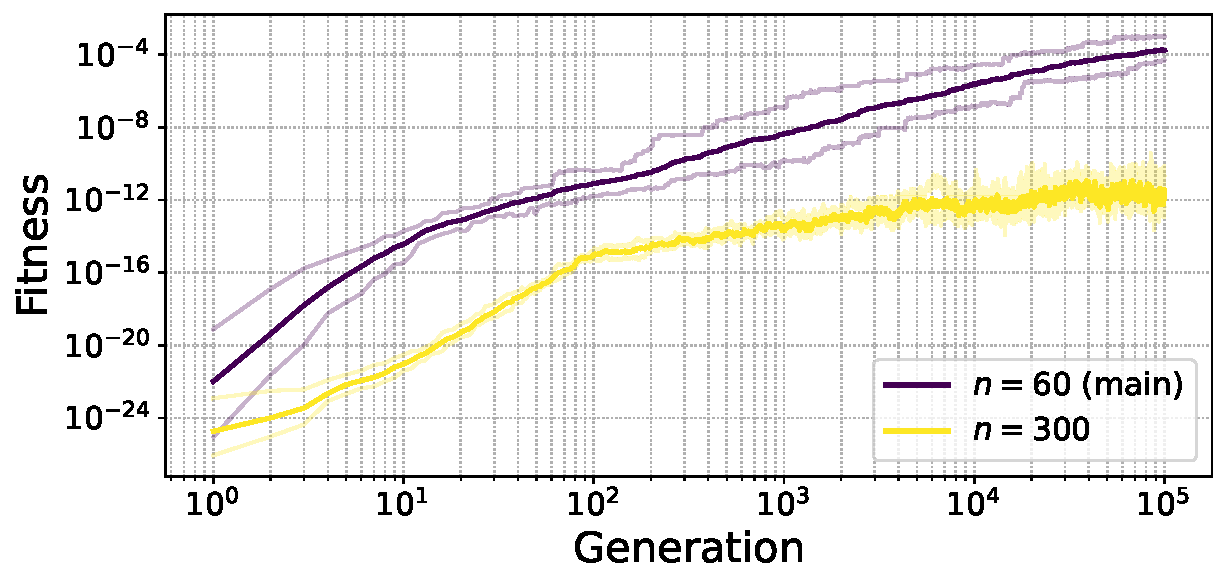
\includegraphics[width=0.75\textwidth]{param/300-genes/fitness_all_with_main.pdf}
\caption[Average fitness during evolution, with a 300-gene genome]{Average fitness during evolution, with a 300-gene genome.}
\end{figure}


\begin{figure}[H]
\centering
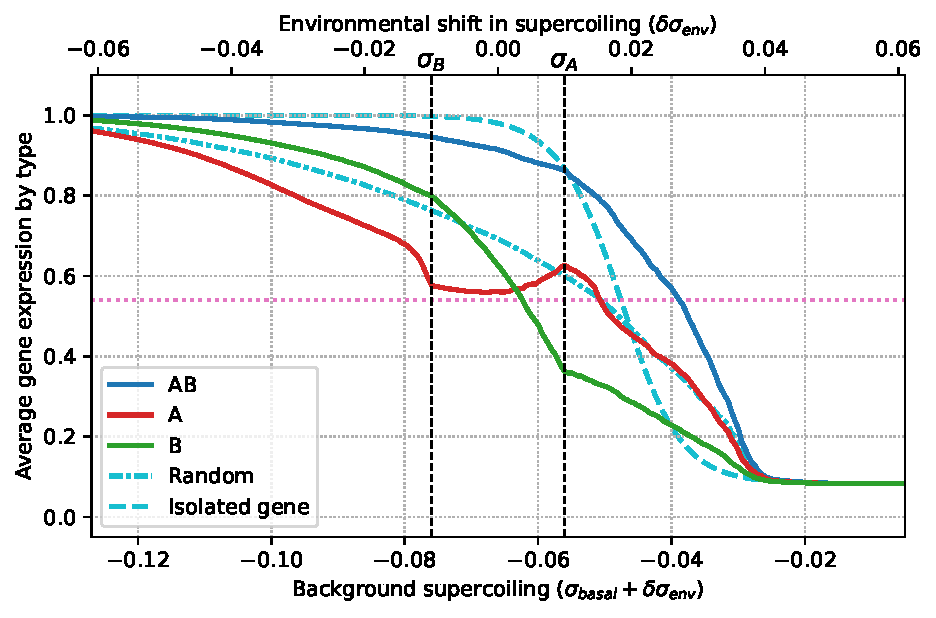
\includegraphics[width=\textwidth]{param/300-genes/activity_sigmas_avg.pdf}
\caption[Average gene expression as a function of background supercoiling, with a 300-gene genome]{Average gene expression as a function of background supercoiling, with a 300-gene genome.}
%\label{fig:param:inter25k-activ-by-sigma}
\end{figure}








\FloatBlock

\section{Mutation in Intergenic Size}


\begin{figure}[H]
  \centering
  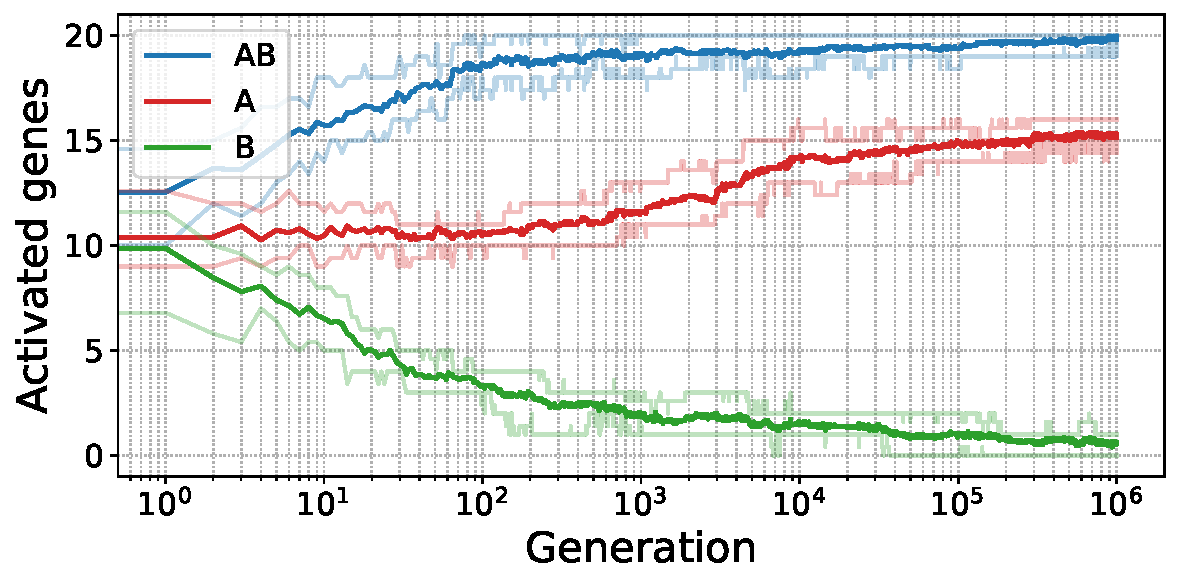
\includegraphics[width=0.49\textwidth]{param/evolve-intergene/gene_activity_env_A.pdf}
  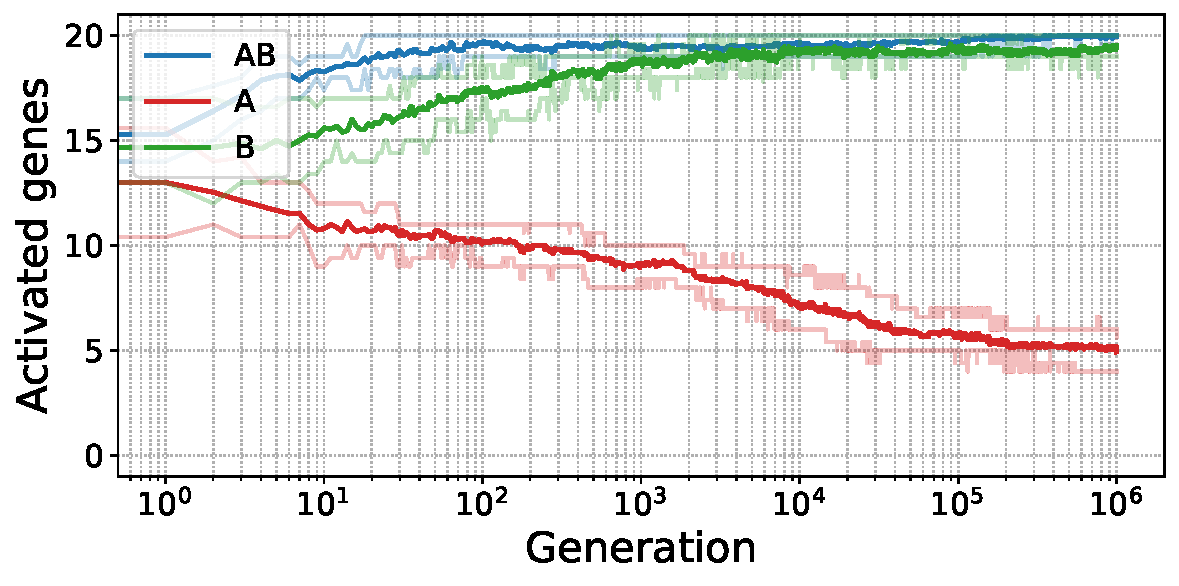
\includegraphics[width=0.49\textwidth]{param/evolve-intergene/gene_activity_env_B.pdf}
  \caption[Evolution of the number of active genes in each environment, with intergenic distance mutations]{Evolution of the number of active genes in environment A (top) and environment B (bottom), with intergenic distance mutations.}
  %\label{fig:param:inter25k-active}
  \end{figure}


\begin{figure}
\begin{elasticrow}[width=\textwidth]
\elasticfigure{param/evolve-intergene/fitness_all_with_main.pdf}
\elasticfigure{param/evolve-intergene/intergenic_size_all.pdf}
\end{elasticrow}
\caption[Average fitness and intergenic size during evolution, with intergenic distance mutations]{Fitness and average genome size during evolution, with intergenic distance mutations.}
\end{figure}



\begin{figure}
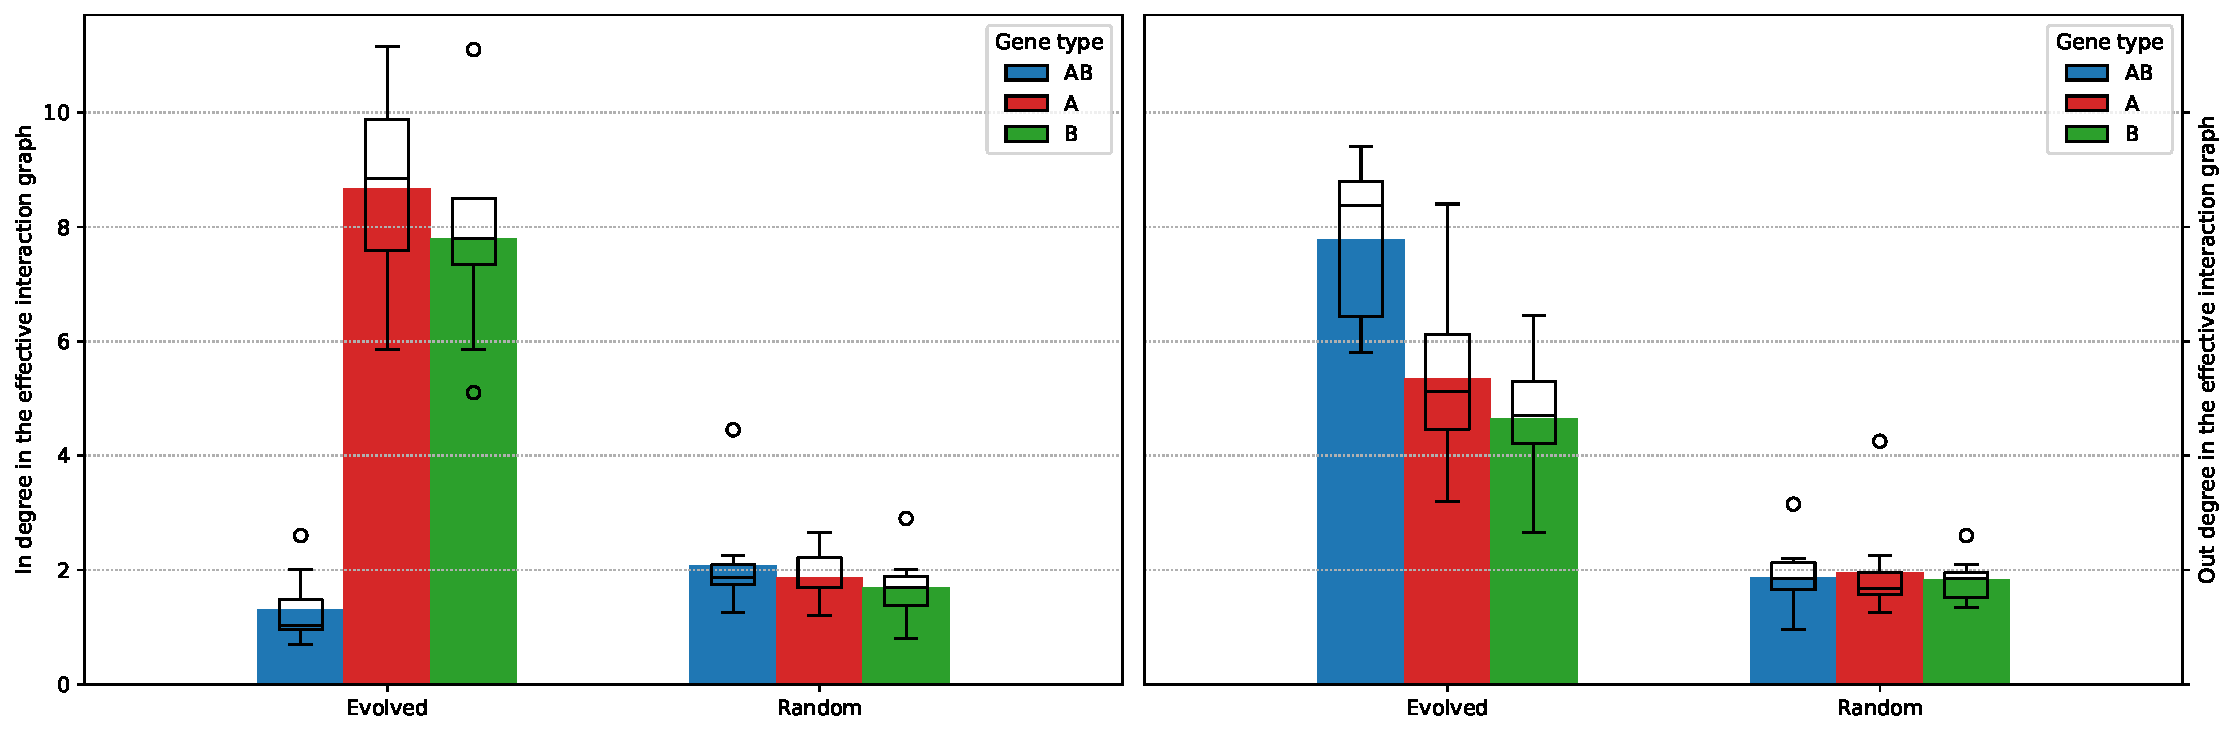
\includegraphics[width=\textwidth]{param/evolve-intergene/effective_graph_combined_degree.pdf}
\caption{Effective graph degrees at the end of evolution with intergenic distance mutations.}
\end{figure}

%\section{Mutation in Basal Supercoiling}